\chapter{Application Design}
\label{cha:design}

After defining the mechanisms which will be implemented, in a next step, the general application flow will be described, as well as offering insight into the user experience design of the parts of the application.

\section{Application Flow}
The flow and usage of the application is separated into two parts: the creation and authoring of the presentation and giving the presentation. Because the technical details of how slide decks are composed are covered in chapter \ref{cha:implementation}, this chapter focuses on the user interface and interaction design of the software from the speaker's and the audience's point of view, during the presentation.

The slides are generally served either from a publicly accessible server or, if all participants are in the same network, locally from the presenter's computer. This means, at the beginning of the presentation, all attendees have to navigate their personal devices' browsers to the set up address (usually a combination of IP address and port). To make this step easier, QR codes pointing to the address can be shown on the first slide or e-mails can be sent out to all participants before the start of the presentation.

% ADD PERSONAS AND REAL WORLD EXAMPLE
The software supports three different modes out of the box: listener, speaker and projector mode. Depending on the mode, a certain set of features is activated, allowing the presenter to have a different interface and more controls than the listeners. Modes are activated via query parameters in the url: The speaker navigates the browser of the device connected to the projector to the url of the presentation and adds the query parameter \printtt{mode=projector}. On his or her personal device, the mode is set to \printtt{speaker}. If no query parameter is given, the application defaults to the listener mode. The presentation software developed prior to the start of the thesis project generally offers a two-dimensional slide space, consisting of master slides (left to right) and subslides (top to bottom). Devices in speaker mode can remote-control the presentation and navigate through said slides. All other devices are synchronised with the state of the presenter and automatically follow along in real-time.

% Base CSS: responsive, if content is too big, everything is uniformly scaled.

% Application Flow, Modes, How does the application work in general?
% Design aspects, sketches, wireframes, thoughts and überlegungen behind design details

\section{General Interface Design}
The general requirement for the interface of the application was to work in all three modes, on any device, from mobile phones to desktops and projectors. When in projector mode, only the content of the current slide, as well as listener reactions are shown (see figure \ref{fig:design-interface-projector}). In listener mode, the interface is a lot richer and additionally features buttons for sharing media, links and asking questions, as well as six different reactions (see figure \ref{fig:design-interface-listener}), which will be discussed in more detail shortly. It also offers small buttons to click on, to navigate between slides. The speaker interface is the most intricate: Besides showing the current slide, it also includes a smaller preview of the upcoming slides in $x$ (master slide) and $y$ (subslide) direction, as well as speaker notes. Additionally there are buttons to mute incoming requests (media, link and questions) and to create new polls (see figure \ref{fig:design-interface-presenter}).

\begin{figure}
\centering
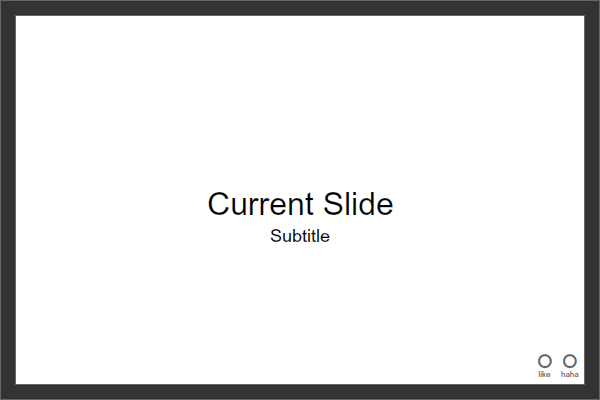
\includegraphics[width=.65\textwidth]{wireframes/projector-interface-projector}
\caption{Wireframe of slide in projector mode, as seen on a projector. No visual controls are shown, only the current slide and listener reactions (lower right corner) are displayed. The presentation progresses through the presenter mode's remote controlling feature.}
\label{fig:design-interface-projector}
\end{figure}

\begin{figure}
\centering\small
\begin{tabular}{cc}
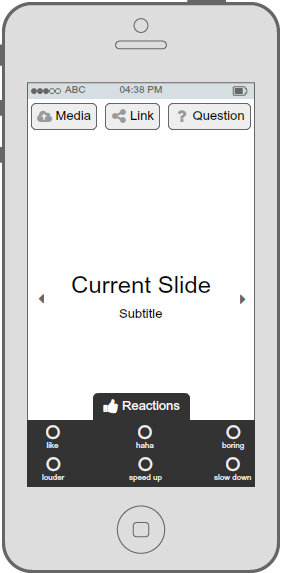
\includegraphics[width=.214\textwidth]{wireframes/listener-interface-mobile} &
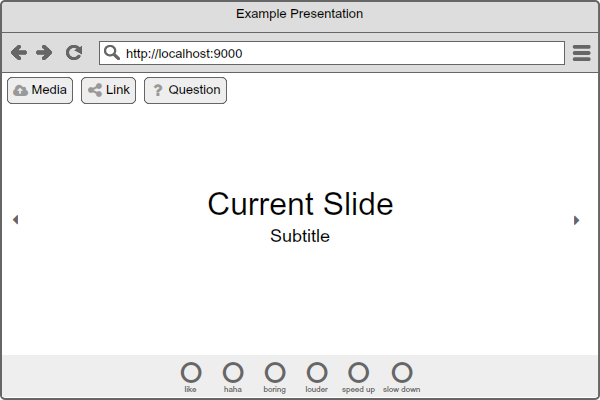
\includegraphics[width=.65\textwidth]{wireframes/listener-interface-desktop}\\
(a) & (b)
\end{tabular}
\caption{Wireframes of general interface in listener mode for (a) mobile phones and (b) desktops. Both offer buttons to share media, links and questions with the presenter, arrow buttons to navigate through the presentation and a possibility to react to the current slide (see section \ref{} for details).}
\label{fig:design-interface-listener}
\end{figure}

\begin{figure}
\centering\small
\begin{tabular}{cc}
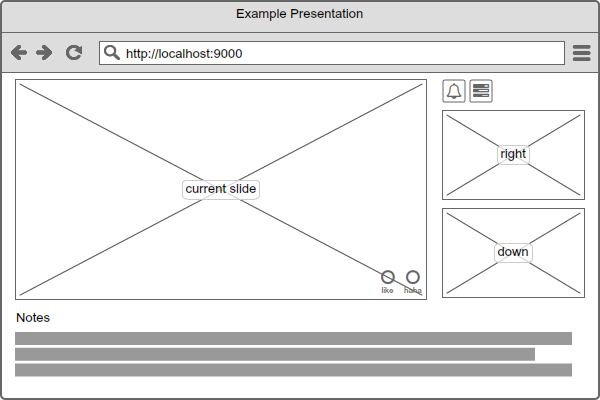
\includegraphics[width=.65\textwidth]{wireframes/presenter-interface-desktop} &
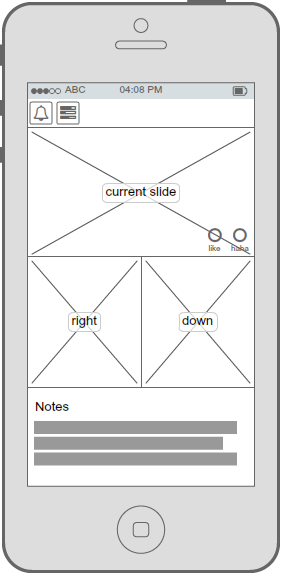
\includegraphics[width=.214\textwidth]{wireframes/presenter-interface-mobile}\\
(a) & (b)
\end{tabular}
\caption{Wireframes of general interface in presenter mode for (a) desktops and (b) mobile phones. The interface consists of a preview of the current slide, the next main slide (\emph{right}) and the next subslide (\emph{down}), as well as showing presenter notes. It also offers buttons to toggle muting of incoming requests and creation of new polls (upper left corner in (a), top in right column in (b)).}
\label{fig:design-interface-presenter}
\end{figure}

\section{General Interaction Principles}
As far as the interaction design of the application is concerned, the main requirement technically is for all state changes to take immediate effect or in other words, for the software to work in real-time. This is true for interactions with the server as well as all internal state changes within the application. All transitions and animations last $200$ms, a value which is both usable on mobile phones and desktops and ``fast enough that it doesn't cause waiting, but slow enough that the transition can be understood'' \cite{GoogleMaterialDesignGuide}. An easing curve with low outgoing and high incoming velocity is used.


% how can we interact? swipe/arrow keys etc., explain modals, hover states etc.


% As described before, it is important for the presenter to be in full control of all mechanisms --> make it easy to add or remove them and to configure!

% Wacker: research has shown that technological problems are the main reason for negative presentation experiences for the speaker. ``Therefore, presentation software should take special care to avoid technological problems and assist the presenter if they should occur''

% We believe it is still important for the speaker to have an overview of the current slide as well as upcoming ones and be able to see notes on the presenter interface

% General requirements: be viewable on every device, work in real-time!

% Emojis
% Find more studies about this! think: facebook, the conference Paulo went to etc. (maybe add photo of audience showing emoji faces!)
% It is therefore important to provide more detailed feedback. Following the evaluation in \cite{Teevan:MobileFeedbackDuringPresentation}, the mechanism proposed in this thesis offers three emotions (approval, laughter, boredom) and three request types (louder, speed up, slow down).

% Polls: Describe why freeze navigation while voting and only allow voting when started by presenter